\documentclass[border=2mm]{standalone}
\usepackage{tikz}
\usepackage{pgfplots}
\usepackage{amsmath}
\pgfplotsset{compat=1.18}

% Definición de colores según paleta del análisis
\definecolor{pais1color}{HTML}{00BFFF}  % Cyan - País 1
\definecolor{pais2color}{HTML}{000000}  % Negro - País 2
\definecolor{pais3color}{HTML}{CC6600}  % Naranja/marrón - País 3
\definecolor{pais4color}{HTML}{0066CC}  % Azul - País 4
\definecolor{pais5color}{HTML}{FF9900}  % Naranja - País 5
\definecolor{gridcolor}{HTML}{CCCCCC}   % Gris claro - Grilla

\begin{document}
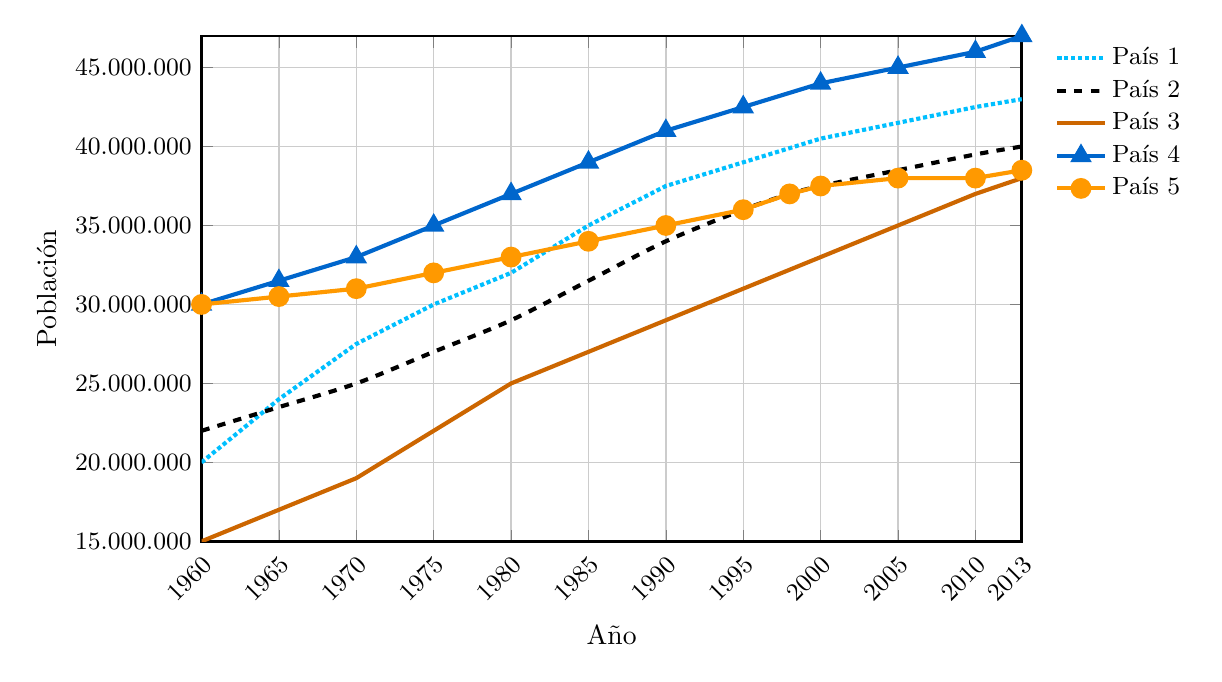
\begin{tikzpicture}
\begin{axis}[
    width=12cm,
    height=8cm,
    xlabel={Año},
    ylabel={Población},
    xmin=1960, xmax=2013,
    ymin=15000000, ymax=47000000,
    xtick={1960,1965,1970,1975,1980,1985,1990,1995,2000,2005,2010,2013},
    xticklabels={1960,1965,1970,1975,1980,1985,1990,1995,2000,2005,2010,2013},
    xticklabel style={rotate=45, anchor=north east, font=\small},
    ytick={15000000,20000000,25000000,30000000,35000000,40000000,45000000},
    yticklabels={15.000.000,20.000.000,25.000.000,30.000.000,35.000.000,40.000.000,45.000.000},
    yticklabel style={font=\small},
    scaled y ticks=false,
    grid=both,
    grid style={gridcolor, line width=0.5pt},
    legend pos=outer north east,
    legend style={font=\small, draw=none},
    legend cell align={left},
    axis lines=box,
    axis line style={black, line width=1pt},
]

% País 1 - Línea punteada cyan - crece linealmente de 20M a 43M
\addplot[
    color=pais1color,
    line width=1.5pt,
    densely dotted,
    mark=none,
] coordinates {
    (1960, 20000000)
    (1965, 24000000)
    (1970, 27500000)
    (1975, 30000000)
    (1980, 32000000)
    (1985, 35000000)
    (1990, 37500000)
    (1995, 39000000)
    (2000, 40500000)
    (2005, 41500000)
    (2010, 42500000)
    (2013, 43000000)
};
\addlegendentry{País 1}

% País 2 - Línea discontinua negra
\addplot[
    color=pais2color,
    line width=1.5pt,
    dashed,
    mark=none,
    smooth,
] coordinates {
    (1960, 22000000)
    (1965, 23500000)
    (1970, 25000000)
    (1975, 27000000)
    (1980, 29000000)
    (1985, 31500000)
    (1990, 34000000)
    (1995, 36000000)
    (1998, 37000000)
    (2000, 37500000)
    (2005, 38500000)
    (2010, 39500000)
    (2013, 40000000)
};
\addlegendentry{País 2}

% País 3 - Línea sólida naranja/marrón - Crecimiento continuo de 15M a 38M
\addplot[
    color=pais3color,
    line width=1.5pt,
    solid,
    mark=none,
] coordinates {
    (1960, 15000000)
    (1965, 17000000)
    (1970, 19000000)
    (1975, 22000000)
    (1980, 25000000)
    (1985, 27000000)
    (1990, 29000000)
    (1995, 31000000)
    (2000, 33000000)
    (2005, 35000000)
    (2010, 37000000)
    (2013, 38000000)
};
\addlegendentry{País 3}

% País 4 - Línea sólida azul con triángulos
\addplot[
    color=pais4color,
    line width=1.5pt,
    solid,
    mark=triangle*,
    mark size=3pt,
    mark options={fill=pais4color, draw=pais4color},
] coordinates {
    (1960, 30000000)
    (1965, 31500000)
    (1970, 33000000)
    (1975, 35000000)
    (1980, 37000000)
    (1985, 39000000)
    (1990, 41000000)
    (1995, 42500000)
    (2000, 44000000)
    (2005, 45000000)
    (2010, 46000000)
    (2013, 47000000)
};
\addlegendentry{País 4}

% País 5 - Línea sólida naranja con círculos
\addplot[
    color=pais5color,
    line width=1.5pt,
    solid,
    mark=*,
    mark size=3pt,
    mark options={fill=pais5color, draw=pais5color},
] coordinates {
    (1960, 30000000)
    (1965, 30500000)
    (1970, 31000000)
    (1975, 32000000)
    (1980, 33000000)
    (1985, 34000000)
    (1990, 35000000)
    (1995, 36000000)
    (1998, 37000000)
    (2000, 37500000)
    (2005, 38000000)
    (2010, 38000000)
    (2013, 38500000)
};
\addlegendentry{País 5}

\end{axis}
\end{tikzpicture}
\end{document}
